\documentclass{standalone}
\usepackage{tikz}
\usetikzlibrary{patterns, positioning}

\begin{document}
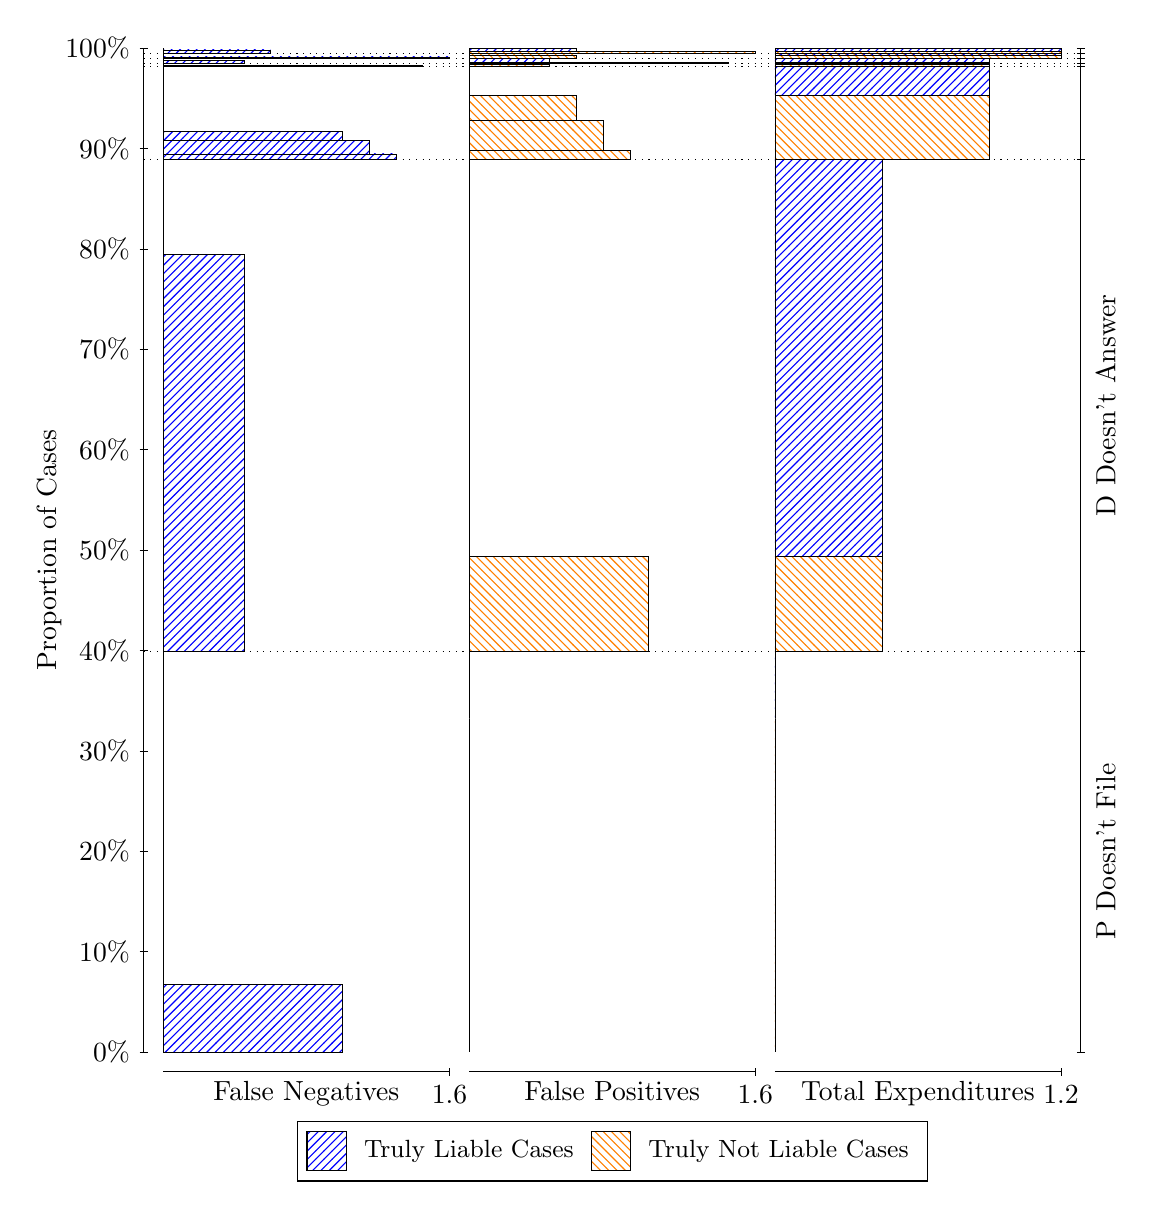
\begin{tikzpicture}
\draw[black, very thin] (1.5,1.75) -- (1.5,14.5);
\node[rotate=90, anchor=center] at (0.3, 8.125) {Proportion of Cases};
\draw[black, very thin] (1.45,1.75) -- (1.55,1.75);
\node[anchor=east] at (1.45, 1.75) {0\%};
\draw[black, very thin] (1.45,3.025) -- (1.55,3.025);
\node[anchor=east] at (1.45, 3.025) {10\%};
\draw[black, very thin] (1.45,4.3) -- (1.55,4.3);
\node[anchor=east] at (1.45, 4.3) {20\%};
\draw[black, very thin] (1.45,5.575) -- (1.55,5.575);
\node[anchor=east] at (1.45, 5.575) {30\%};
\draw[black, very thin] (1.45,6.85) -- (1.55,6.85);
\node[anchor=east] at (1.45, 6.85) {40\%};
\draw[black, very thin] (1.45,8.125) -- (1.55,8.125);
\node[anchor=east] at (1.45, 8.125) {50\%};
\draw[black, very thin] (1.45,9.4) -- (1.55,9.4);
\node[anchor=east] at (1.45, 9.4) {60\%};
\draw[black, very thin] (1.45,10.675) -- (1.55,10.675);
\node[anchor=east] at (1.45, 10.675) {70\%};
\draw[black, very thin] (1.45,11.95) -- (1.55,11.95);
\node[anchor=east] at (1.45, 11.95) {80\%};
\draw[black, very thin] (1.45,13.225) -- (1.55,13.225);
\node[anchor=east] at (1.45, 13.225) {90\%};
\draw[black, very thin] (1.45,14.5) -- (1.55,14.5);
\node[anchor=east] at (1.45, 14.5) {100\%};

\draw[black, very thin] (13.4,1.75) -- (13.4,14.5);
\draw[black, very thin] (13.35,1.75) -- (13.45,1.75);
\node[anchor=west] at (13.35, 1.75) {};
\draw[black, very thin] (13.35,6.8406) -- (13.45,6.8406);
\node[anchor=west] at (13.35, 6.8406) {};
\draw[black, very thin] (13.35,13.083) -- (13.45,13.083);
\node[anchor=west] at (13.35, 13.083) {};
\draw[black, very thin] (13.35,14.266) -- (13.45,14.266);
\node[anchor=west] at (13.35, 14.266) {};
\draw[black, very thin] (13.35,14.304) -- (13.45,14.304);
\node[anchor=west] at (13.35, 14.304) {};
\draw[black, very thin] (13.35,14.364) -- (13.45,14.364);
\node[anchor=west] at (13.35, 14.364) {};
\draw[black, very thin] (13.35,14.436) -- (13.45,14.436);
\node[anchor=west] at (13.35, 14.436) {};
\draw[black, very thin] (13.35,14.5) -- (13.45,14.5);
\node[anchor=west] at (13.35, 14.5) {};

\draw[black, very thin, pattern color=blue, pattern=north east lines] (1.75,1.75) rectangle (4.0208,2.6054);
\draw[black, very thin, pattern color=orange, pattern=north west lines] (1.75,2.6054) rectangle (1.75,6.8406);
\draw[black, very thin, pattern color=blue, pattern=north east lines] (1.75,6.8406) rectangle (2.7719,11.88);
\draw[black, very thin, pattern color=orange, pattern=north west lines] (1.75,11.88) rectangle (1.75,13.083);
\draw[black, very thin, pattern color=blue, pattern=north east lines] (1.75,13.083) rectangle (4.7021,13.155);
\draw[black, very thin, pattern color=blue, pattern=north east lines] (1.75,13.155) rectangle (4.3615,13.326);
\draw[black, very thin, pattern color=blue, pattern=north east lines] (1.75,13.326) rectangle (4.0208,13.446);
\draw[black, very thin, pattern color=orange, pattern=north west lines] (1.75,13.446) rectangle (1.75,14.266);
\draw[black, very thin, pattern color=blue, pattern=north east lines] (1.75,14.266) rectangle (5.0427,14.277);
\draw[black, very thin, pattern color=orange, pattern=north west lines] (1.75,14.277) rectangle (1.75,14.304);
\draw[black, very thin, pattern color=blue, pattern=north east lines] (1.75,14.304) rectangle (2.7719,14.346);
\draw[black, very thin, pattern color=orange, pattern=north west lines] (1.75,14.346) rectangle (1.75,14.364);
\draw[black, very thin, pattern color=blue, pattern=north east lines] (1.75,14.364) rectangle (5.3833,14.387);
\draw[black, very thin, pattern color=orange, pattern=north west lines] (1.75,14.387) rectangle (1.75,14.436);
\draw[black, very thin, pattern color=blue, pattern=north east lines] (1.75,14.436) rectangle (3.1125,14.477);
\draw[black, very thin, pattern color=orange, pattern=north west lines] (1.75,14.477) rectangle (1.75,14.5);
\draw[black, very thin, pattern color=orange, pattern=north west lines] (5.6333,1.75) rectangle (5.6333,5.9852);
\draw[black, very thin, pattern color=blue, pattern=north east lines] (5.6333,5.9852) rectangle (5.6333,6.8406);
\draw[black, very thin, pattern color=orange, pattern=north west lines] (5.6333,6.8406) rectangle (7.9042,8.044);
\draw[black, very thin, pattern color=blue, pattern=north east lines] (5.6333,8.044) rectangle (5.6333,13.083);
\draw[black, very thin, pattern color=orange, pattern=north west lines] (5.6333,13.083) rectangle (7.6771,13.204);
\draw[black, very thin, pattern color=orange, pattern=north west lines] (5.6333,13.204) rectangle (7.3365,13.578);
\draw[black, very thin, pattern color=orange, pattern=north west lines] (5.6333,13.578) rectangle (6.9958,13.903);
\draw[black, very thin, pattern color=blue, pattern=north east lines] (5.6333,13.903) rectangle (5.6333,14.266);
\draw[black, very thin, pattern color=orange, pattern=north west lines] (5.6333,14.266) rectangle (6.6552,14.293);
\draw[black, very thin, pattern color=blue, pattern=north east lines] (5.6333,14.293) rectangle (5.6333,14.304);
\draw[black, very thin, pattern color=orange, pattern=north west lines] (5.6333,14.304) rectangle (8.926,14.322);
\draw[black, very thin, pattern color=blue, pattern=north east lines] (5.6333,14.322) rectangle (6.6552,14.364);
\draw[black, very thin, pattern color=orange, pattern=north west lines] (5.6333,14.364) rectangle (6.9958,14.413);
\draw[black, very thin, pattern color=blue, pattern=north east lines] (5.6333,14.413) rectangle (5.6333,14.436);
\draw[black, very thin, pattern color=orange, pattern=north west lines] (5.6333,14.436) rectangle (9.2667,14.46);
\draw[black, very thin, pattern color=blue, pattern=north east lines] (5.6333,14.46) rectangle (6.9958,14.5);
\draw[black, very thin, pattern color=orange, pattern=north west lines] (9.5167,1.75) rectangle (9.5167,5.9852);
\draw[black, very thin, pattern color=blue, pattern=north east lines] (9.5167,5.9852) rectangle (9.5167,6.8406);
\draw[black, very thin, pattern color=orange, pattern=north west lines] (9.5167,6.8406) rectangle (10.879,8.044);
\draw[black, very thin, pattern color=blue, pattern=north east lines] (9.5167,8.044) rectangle (10.879,13.083);
\draw[black, very thin, pattern color=orange, pattern=north west lines] (9.5167,13.083) rectangle (12.242,13.903);
\draw[black, very thin, pattern color=blue, pattern=north east lines] (9.5167,13.903) rectangle (12.242,14.266);
\draw[black, very thin, pattern color=orange, pattern=north west lines] (9.5167,14.266) rectangle (12.242,14.293);
\draw[black, very thin, pattern color=blue, pattern=north east lines] (9.5167,14.293) rectangle (12.242,14.304);
\draw[black, very thin, pattern color=orange, pattern=north west lines] (9.5167,14.304) rectangle (12.242,14.322);
\draw[black, very thin, pattern color=blue, pattern=north east lines] (9.5167,14.322) rectangle (12.242,14.364);
\draw[black, very thin, pattern color=orange, pattern=north west lines] (9.5167,14.364) rectangle (13.15,14.413);
\draw[black, very thin, pattern color=blue, pattern=north east lines] (9.5167,14.413) rectangle (13.15,14.436);
\draw[black, very thin, pattern color=orange, pattern=north west lines] (9.5167,14.436) rectangle (13.15,14.46);
\draw[black, very thin, pattern color=blue, pattern=north east lines] (9.5167,14.46) rectangle (13.15,14.5);
\draw[black, dotted] (1.5,6.8406) -- (13.4,6.8406);
\draw[black, dotted] (1.5,13.083) -- (13.4,13.083);
\draw[black, dotted] (1.5,14.266) -- (13.4,14.266);
\draw[black, dotted] (1.5,14.304) -- (13.4,14.304);
\draw[black, dotted] (1.5,14.364) -- (13.4,14.364);
\draw[black, dotted] (1.5,14.436) -- (13.4,14.436);
\draw[black, very thin] (1.75,1.5) -- (5.3833,1.5);
\node[anchor=north] at (3.5667, 1.5) {False Negatives};
\draw[black, very thin] (5.3833,1.45) -- (5.3833,1.55);
\node[anchor=north] at (5.3833, 1.45) {1.6};

\draw[black, very thin] (5.6333,1.5) -- (9.2667,1.5);
\node[anchor=north] at (7.45, 1.5) {False Positives};
\draw[black, very thin] (9.2667,1.45) -- (9.2667,1.55);
\node[anchor=north] at (9.2667, 1.45) {1.6};

\draw[black, very thin] (9.5167,1.5) -- (13.15,1.5);
\node[anchor=north] at (11.333, 1.5) {Total Expenditures};
\draw[black, very thin] (13.15,1.45) -- (13.15,1.55);
\node[anchor=north] at (13.15, 1.45) {1.2};

\node[black, centered, rotate=90] at (13.72, 4.2953) {P Doesn't File};
\node[black, centered, rotate=90] at (13.72, 9.962) {D Doesn't Answer};






\draw (7.449999999999999,1.5) node[draw=none] (baseCoordinate) {};
\begin{scope}[align=center]
        \matrix[scale=0.5, draw=black, below=0.5cm of baseCoordinate, nodes={draw}, column sep=0.1cm]{
            \node[rectangle, draw, minimum width=0.5cm, minimum height=0.5cm, pattern=north east lines, pattern color=blue] {}; &
            \node[draw=none, font=\small] (B) {Truly Liable Cases}; &
            \node[rectangle, draw, minimum width=0.5cm, minimum height=0.5cm, pattern=north west lines, pattern color=orange] {}; &
            \node[draw=none, font=\small] (B) {Truly Not Liable Cases}; \\
            };
\end{scope}

\end{tikzpicture}
\end{document}